
% This LaTeX was auto-generated from MATLAB code.
% To make changes, update the MATLAB code and republish this document.

\documentclass{article}
\usepackage{graphicx}
\usepackage{color}

\sloppy
\definecolor{lightgray}{gray}{0.5}
\setlength{\parindent}{0pt}

\begin{document}

    
    \begin{verbatim}
function [] = ContourPlot()
    clf
    clear
    [Qw, D] = meshgrid(0.01:0.001:0.2,0.1:0.001:0.3);%0.00001:0.0001:0.0008

    %Qw = 0.1128;
    %D = 0.1818;
    d = 0.0005;

    %Analysis Variables
    gamma = 168.5; %lbm/ft3 - limestone density
    L = 15*5280; %feet - length of pipeline
    W = 12.67; %lbm/sec - mass flowrate of limestone
    a = 0.01; %ft. - average lump size of limestone before grinding
    g = 32.17; %ft/sec^2 - acceleration due to gravity
    gc = 32.17; % lbmft/lbfsec^2 - conversion between lbf and lbm
    pw = 62.4; %lbm/ft3 - density of water
    mew = 7.392*10^-4;%lbm/(ft-sec) - viscosity of water

    %Analysis Functions
    Area = pi.*D.^2./4; %ft^2 - cross sectional area of pipe
    Ql = W./gamma; %ft^3/sec - flowrate of limestone
    Q = Ql+Qw; %ft^3/sec - total slurry flow rate
    V = Q./Area; %ft/sec - average flow velocity
    c = Ql./(Q); % volumetric concentration of slurry
    S=gamma./pw; % specific gravity of the limestone

    Rw = (pw.*V.*D)./mew;
    if Rw<10^5
    fw = 0.3164./Rw.^0.25; % friction factor of water
    else
    fw = 0.0032+0.221*Rw.^-0.237; % friction factor of water
    end
    CdRp2 = 4*g.*pw.*d.^3.*((gamma-pw)./(3.*mew^2));
    % Curve fit is from JMP 14.
    a1 = 0.421534;
    b1= 104.95427;
    h1 = 0.5679997;
    d1 = 508.55715;
    f1 = 1.2131968;
    Cd = a1+b1*exp(-h1*log(CdRp2))+d1*exp(-f1*log(CdRp2));% average drag coefficient of the particles

    p = pw + c.*(gamma-pw); % density of slurry lbm/ft^3

    f = fw.*(pw./p+150.*c.*(pw./p).*((g.*D.*(S-1))./(V.^2.*sqrt(Cd))).^1.5);

    Pg = 218*W.*(1./sqrt(d)-1./sqrt(a)); %ftlbf/sec - Power for grinding
    GrindingPowerHP = Pg/550;

    changep = f.*p.*L.*V.^2./(D.*2.*gc);
    Pf = changep.*Q; %ft-lbf/sec - Friction power loss
    PumpingPowerHP = Pf./550;

    Vc = (40.*g.*c.*(S-1).*D./sqrt(Cd)).^0.5;

    PlantOperationHoursPerYear = 8.*300; %hours per year
    CostOfEnergy = 0.07; %cost per horsepowerhour
    InitialCostGrinder = GrindingPowerHP*300;
    InitialCostPump = PumpingPowerHP*200;
    CostPerYear = PlantOperationHoursPerYear.*(PumpingPowerHP+GrindingPowerHP).*CostOfEnergy;
    InitialCost = InitialCostGrinder+InitialCostPump;
    i = 0.07;
    n = 7;
    NetPresentCost = InitialCost+(CostPerYear.*((1+i)^n-1)/(i*(1+i)^n));

    arg1 = Qw;
    arg2 = D;

    figure(1)
    [C,h] = contour(arg1,arg2,NetPresentCost,[430000,440000,457012.9,470000,480000,600000,700000],'b-');
    clabel(C,h,'Labelspacing',250);
    title('Pipeline Contour Plot');
    xlabel('Water Flow Rate');
    ylabel('Inner Pipe Diameter');
    hold on;

    contour(arg1,arg2,1.1*Vc-V,[0,0],'r-','LineWidth',2);
    contour(arg1,arg2,c-0.4,[0,0],'m-','LineWidth',2);

    legend('Net Present Value','V>1.1*Vc','c<0.4')

end
\end{verbatim}

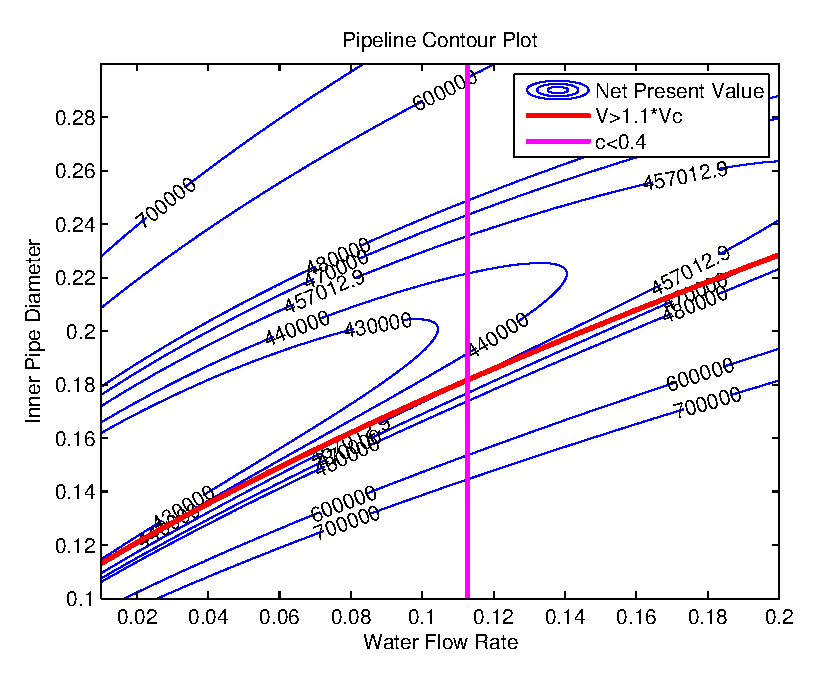
\includegraphics [width=4in]{ContourPlot_01.eps}



\end{document}
    
